\documentclass[]{beamer}
\usepackage{beamerthemesplit}
\usepackage{radoslav-beamer}

\usepackage{pgfplots}
\pgfplotsset{compat=newest}
\usetikzlibrary{pgfplots.groupplots}
\usetikzlibrary{positioning}

\usetheme{CambridgeUS}

\title{Examples of Implicitization of Hypersurfaces}
\author{Radoslav Zlatev}
\institute{Cornell University}
\date{June 4, 2015}

\begin{document}



\begin{frame}
\titlepage
\end{frame}



\section{Intro}

\begin{frame}
Let $X$ be a smooth projective toric variety of dimension $n-1$.
Let $S,\mathfrak{n}$ be its Cox ring and irrelevant ideal
and $\L=\O_X(\e)$ be a line bundle on $X$ such that $h^0(\L)>n$.

Let $\phi_0,\ldots,\phi_n\in H^0(X,\L)$ be linearly independent
such that the induced
\[
	\phi=(\phi_0,\ldots,\phi_n):X\To\PP^n_{x_0,\ldots,x_n}
\]
is generically finite onto its image.
Then the closed image $Y$ is irreducible hypersurface and so
defined by a single polynomial over the $x_j$.
% scheme-theoretic image $Y$ of $\phi$ is reduced and irreducible
% and coincides with the closure of the image of the set-theoretic map $\phi$
% on closed points.

\begin{definition}
	The implicitization problem, as we shall study it, is the problem of finding
	the {\em implicit equation} $P(\x)$ defining $Y\se\PP^n$ when given the coordinate
	functions $\phi_j$.
	More generally, it is concerned with the relation between the algebraic propeprties
	of the (ideal of the) $\phi_j$ in $S$ and the geometric properties of $Y$ in $\PP^n$.
\end{definition}
\end{frame}

\begin{frame}
	Problems with standard method:
	\begin{itemize}
	\item the problem can be solved by Gr\"obner bases but often this is not computationally feasible
	\item geometrically, GB are a black box which neither makes use of nor gives insight
	\end{itemize}
	
	Reincarnation: CAD
	\begin{itemize}
	\item Tomas Sederberg and Falai Chen, "Implicitization using moving curves and surfaces", 1995
	\item David Cox, Ronald Goldman, and Ming Zhang. "On the validity of implicitization by moving quadrics for rational surfaces with no base points", 2000
	\item Laurent Bus\'e and Jean-Pierre Jouanolou. "On the closed image of a rational map and the implicitization problem", 2003
	\end{itemize}
\end{frame}


\section{Setup}

\begin{frame}
Fix a rational map $\phi$ as described before, and let
\[
	\phi_0,\ldots,\phi_n\in H^0(X,\O_X(\e))
\]
be its $n+1$ linearly independent coordinates.

We say that a degree-$(\d,i)$ form $g(s_0,\ldots,s_m;x_0,\ldots,x_n)$ in $S[\x]$ is
a syzygy on $\phi$ over degree $\d$ if
\[
	g(s_0,\ldots,s_m;\phi_0,\ldots,\phi_n)=0
\]
as an identity in $S$.

The syzygies on $\phi$ over any $\d$ form a finite graded sub-$\CC[\x]$-module of $S[\x]$.
We denote this submodule by $\I_{\d,\bullet}$.
\end{frame}

\begin{frame}
Let
\[
	\{g_1,\ldots,g_\mu\}
\]
be a minimal set of homogeneneous generators for the syzygies module $\I_{\d,\bullet}$,
for some given fixed $\phi$ and $\d$.

Let
\[
	\basis(S_\d)
\]
be an $r$-row-matrix of the basis of $\CC$-vector space basis of $S_\d$ in some fixed
monomial order. For example, for $X=\PP^2$ so that $S=\CC[s_0,s_1,s_2]$, $\d=2$
and the lexicographic order, we get
\[
	\basis(S_3)=\begin{bmatrix}s_0^2& s_0s_1& s_0s_2& s_1^2& s_1s_2& s_2^2\end{bmatrix}
\]
which is an $(r=\dim_\CC(S_\d)=6)$-row vector over $S$ and $S[\x]$.
\end{frame}

\begin{frame}
Given the generating set $\{g_1,\ldots,g_\mu\}$ of $\I_{\d,\bullet}$,
we take $N$ to be the coefficient matrix such that
\[
	\basis(S_\d)\cdot N=\begin{bmatrix}g_1& \ldots& g_\mu\end{bmatrix}
\]

For example, given the syzygies
\[
	% \phi=(s_0^3,s_1^2s_2,s_0^2s_1+s_2^3,s_0s_1s_2):\PP^2\To\PP^3
	\{s_0x_1-s_1x_3, s_2x_0x_1-s_0x_3^2\}
\]
over degree $\d=1$ on a rational map with source $\PP^2$, we get
\[
	\begin{bmatrix}s_0& s_1& s_2\end{bmatrix} \begin{bmatrix}x_1& -x_3^2\\ -x_3& 0\\ 0& x_0x_1\end{bmatrix}=
	\begin{bmatrix}s_0x_1-s_1x_3& s_2x_0x_1-s_0x_3^2\end{bmatrix}
\]
\end{frame}



\section{Results}

% the main theorem
\begin{frame}
\begin{theorem}
	Let $X$ be a smooth projective toric variety of dimension $n-1$
	and $\e\in\Pic(X)$ such that $h^0(\O_X(\e))>n$.
	Let $\phi:X\To\PP^n$ be a rational map given by $n+1$ linearly independent
	global sections of $\O_X(\e)$ such that the base locus $Z\se X$ is 0-dimensional.
	Let $\d\in\reg(B_P)$ be a degree in the regularity of the preimage of $\phi$
	and $N$ be the $r\times\mu$ matrix of syzygies of $\phi$ over $S_\d$. Then
	\[
		\gcd(\minors(r,N))=P^{\deg(\phi)}
	\]
\end{theorem}
% \begin{itemize}
% \item<1-> First item
% \item<2-> Second item
% \item<3-> ...
% \end{itemize}
\end{frame}

\begin{frame}
\begin{theorem}
	Let $X$ be a smooth projective toric variety of dimension $n-1$
	and $\e\in\Pic(X)$ such that $h^0(\O_X(\e))>n$.
	Let $\phi:X\To\PP^n$ be a rational map given by $n+1$ linearly independent
	global sections of $\O_X(\e)$ such that the base locus $Z\se X$ is 0-dimensional.
	Let {\color{red}$\d\in\reg(B_P)$ be a degree in the regularity of the preimage of $\phi$}
	and $N$ be the $r\times\mu$ matrix of syzygies of $\phi$ over $S_\d$. Then
	\[
		{\color{red}\gcd}(\minors(r,N))=P^{\color{red}\deg(\phi)}
	\]
\end{theorem}
\end{frame}

% relaxation of the conditions
\begin{frame}
\begin{theorem}
	Let $X$ be a smooth projective toric variety of dimension $n-1$
	and $\e\in\Pic(X)$ such that $h^0(\O_X(\e))>n$.
	Let $\phi:X\To\PP^n$ be a rational map given by $n+1$ linearly independent
	global sections of $\O_X(\e)$ such that the base locus $Z\se X$ is 0-dimensional.
	Let $\d$ be a degree such that $h^0(\O_X(\d))>0$
	and $N$ be the $r\times\mu$ matrix of syzygies of $\phi$ over $S_\d$. Then
	\[
		\rad(\minors(r,N))=P
	\]
\end{theorem}
\end{frame}

\begin{frame}
\begin{conjecture}
	Let $X$ be a smooth projective toric variety of dimension $n-1$
	and $\e\in\Pic(X)$ such that $h^0(\O_X(\e))>n$.
	Let $\phi:X\To\PP^n$ be a birational map given by $n+1$ linearly independent
	global sections of $\O_X(\e)$.
	Let $\d$ be a degree such that $h^0(\O_X(\d))>0$
	and $N$ be the $r\times\mu$ matrix of syzygies of $\phi$ over $S_\d$. Then
	the multiple-point locus of $\phi$ on its image $Y\se\PP^n$ is given,
	set-theoretically, by
	\[
		\rad(\minors(r-1,N))
	\]
\end{conjecture}
\end{frame}

% the approximation complex
\begin{frame}
\begin{corollary}
	Let $X$ be a smooth projective toric variety of dimension $n-1$
	and $\e\in\Pic(X)$ such that $h^0(\O_X(\e))>n$.
	Let $\phi:X\To\PP^n$ be a rational map given by $n+1$ linearly independent
	global sections of $\O_X(\e)$ such that the base locus $Z\se X$ is 0-dimensional
	and locally complete intersection.
	Let $\d\in\Pic(X)$ be {\em large enough} in the poset of degrees. Then
	\[
		\gcd(\minors(r,N_1))=P^{\deg(\phi)}
	\]
\end{corollary}
\end{frame}

% the method of moving planes and quadrics
\begin{frame}
\begin{corollary}
	Let $X=\PP^2$ and $\phi:X\To\PP^3$ be a morphism given by four linearly independent forms of degree $e$.
	Suppose that there are exactly $e-1$ linear syzygies on $\phi$ over $e-1$.
	Then $N=(N_1~|~N_2)$, $N$ is square and $\phi$ is birational. In particular, up to a unit,
	\[
		\det(N)=\det(N_1~|~N_2)=P(\x)
	\]
\end{corollary}
\end{frame}

\begin{frame}
\begin{corollary}
	Let $X=\PPP$ and $\phi:X\To\PP^3$ be a morphism given by four linearly independent forms of bidegree $\e=(e_1,e_2)$.
	Suppose that there are no linear syzygies on $\phi$ over $\d=(e_1-1,e_2-1)$.
	Then $N_2$ is square, $N=N_2$ and $\phi$ is birational. In particular, up to a unit,
	\[
		\det(N)=\det(N_2)=P(\x)
	\]
\end{corollary}
\end{frame}



\section{Examples}

% example 1
\begin{frame}
\begin{example}
Let $X=\PP^2_{s,t,u}$ and $\phi=(su^2,t^2(s+u),st(s+u),tu(s+u))$. Then $\phi$ is birational onto its
image; the basepoints are $(1,0,0)$, $(0,1,0)$ and $(0,0,1)$,
all ci of multiplicities 2, 3, and 1, respectively. For $\d=1$ we get
\[
N=\bgroup\begin{bmatrix}{-{x}_{3}}&
0&
{x}_{1}&
{-{x}_{3}^{2}}\\
0&
{-{x}_{3}}&
{-{x}_{2}}&
{x}_{0} {x}_{2}+{x}_{0} {x}_{3}\\
{x}_{2}&
{x}_{1}&
0&
0\\
\end{bmatrix}\egroup
\]
and for $\d=2$ we get a $6\times 9$-matrix whose columns are all linear.

The implicit equation is $P(\x)=x_0x_1x_2+x_0x_1x_3-x_2x_3^2$ and
\[
	\gcd(\minors(3,N))=P(\x)
\]
as expected. However $\det(N_1)=0$.
\end{example}
\end{frame}

% example 2
\begin{frame}
\begin{example}
	Let $X=\PPP$ with Cox ring $S=\CC[s,u;t,v]$
	and let $\phi$ be the birational map to $\PP^3$ given by
	\[
		\phi=(s^{2} v^{2},s u v^{2},u^{2} t^{2}+u^{2} t v,s u t v-101 u^{2}t v)
	\]
	Then the base locus of $\phi$ consists of two points, given scheme-theoretically
	by $\la s,t\ra$ and $\la u^2,uv,v^2\ra$.
	The former is a complete intersection point of multiplicity $1$
	and the latter is not---it is of degree $3$ and multiplicity $4$.
	
	The implicit equation, up to a unit, is
	\[
		P(\x)={x}_{0}^{2} {x}_{2}-202 {x}_{0} {x}_{1} {x}_{2}+10201
		{x}_{1}^{2} {x}_{2}-{x}_{0} {x}_{1} {x}_{3}+101 {x}_{1}^{2} {x}_{3}-{x}_{0}
		{x}_{3}^{2}
	\]
\end{example}
\end{frame}

\begin{frame}
\begin{example}[cont]
	Taking $\d=(1,1)$ we get
	\[
		N=\begin{bmatrix}0&
	       {x}_{1}&
	       0&
	       0&
	       {x}_{0} {x}_{2}-{x}_{3}^{2}\\
	       {x}_{2}&
	       {-{x}_{3}}&
	       {-{x}_{1}}&
	       {-{x}_{3}}&
	       {-{x}_{3}^{2}}\\
	       {-{x}_{3}}&
	       {-101 {x}_{1}}&
	       0&
	       {x}_{0}-101 {x}_{1}&
	       -10201 {x}_{1} {x}_{2}-202 {x}_{3}^{2}\\
	       -101 {x}_{2}-{x}_{3}&
	       0&
	       {x}_{0}&
	       0&
	       20402 {x}_{2} {x}_{3}-202 {x}_{3}^{2}\\
	       \end{bmatrix}
	\]
	and
	\[
		\gcd(\minors(4,N))=P(\x)
	\]
	Note that $N_1$ is square and $\det(N_1)=x_1P(\x)$ so $P(\x)=\det(M)$
	where $M$ is the submatrix of $N$ consisting of rows $2,3,4$ and columns $1,3,4$
	but $M$ is not a matrix of syzygies.
\end{example}
\end{frame}

% example 3
\begin{frame}
\begin{example}
	Let $X=\PP^2_{s,t,u}$ and $\phi=(s^5,t^5,su^4,st^2u^2)$.
	Then $\phi$ is generically 2-1 map with the single ci basepoint $(0,0,1)$ of multiplicity 5.
	We have
	\[
		P(\x)=x_0x_1^4x_2^5-x_3^{10}
	\]
	Over $\d=1$ we have
	\[
		N=\begin{bmatrix}x_1x_2& -x_3^8& 0\\ -x_2^3& x_0x_1^3x_2^4& 0\\ 0& 0& x_0x_1^4x_2^5-x_3^{10}\end{bmatrix}
	\]
	and
	\[
		\gcd(\minors(3,N))=\det(N)=P(\x)^2
	\]
\end{example}
\end{frame}

% example 4
\begin{frame}
\begin{lemma}
	Let $Y\se\PP^3$ be a reduced surface of degree $4$ whose singular locus contains 3 nondegenerate concurent lines.
	Then $Y=V(\det(M))$ for some $4\times4$-matrix $M$. $M$ is not a matrix of syzygies.
\end{lemma}
\begin{example}
	Let $X=\PP^1_{s,u}\times\PP^1_{t,v}$ and $\phi_0,\ldots,\phi_3$ be four general linearly independent
	biquadrics with common zero set $V(s^2,st,t^2)$.
	Let $\phi:X\To\PP^3$ be the map given by the $\phi_j$.
	Then $\image(\phi)$ is of degree 4 and singular along 3 nondegenerate concurent lines.
\end{example}
\end{frame}

% example 5
\begin{frame}
\begin{example}
	Let $X=(\PP^1)^3$, $\L=\O_X(2,2,1)$
	and let $\phi_0,\ldots,\phi_4$ be a 5 general linearly independent global sections,
	i.e.
	\[
		\Span_\CC\{\phi_0,\ldots,\phi_4\}\in\mathbb{G}(4,\PP H^0(X,\L))
	\]
	Then $\phi$ is basepoint-free and birational.
	The implicit equation is of degree $24$ on 5 variables, so a Gr\"obner basis
	calculation is unfeasible.
	
	Over $\d=(2,1,1)$ we have $r=\dim_\CC(S_\d)=12$ rows and we expect $N_1$ to be empty
	while $N_2$ to be of size $12\times12$.
	Following our template proof, which now works almost automatically,
	we find that $N=N_2$ is square and $\det(N)=P(\x)$.
\end{example}
\end{frame}

\begin{frame}
\begin{example}[cont]
	Computating the matrices $N_1$ and $N_2$ took less than 1s (0.702681s) on the machines in 103,
	while the computation of the equation itself, i.e. $\det(N)$, took 66m.
	I killed the Gr\"obner bases computataion after a little more than 24h.
\end{example}
\end{frame}



\section{Sketch of Proof}

% step 1
\begin{frame}
\begin{proof}[Step 1]
	\def\qedsymbol{}
	Let $J=\la \phi_0,\ldots,\phi_n\ra\se S$ be the graded ideal of the coordinates of $\phi$.
	Then $V(J)$ is the baselocus of $\phi$.
	Let $R=S[\x]=S\tensor \CC[\x]$ and $\Rees_S(J)$ be the Rees algebra of $J$.
	Then
	\[
		\Rees_S(J)=R/\I
	\]
	where
	\[
		\I=\la \sum_{|\alpha|=i} a_\alpha(\s){\x}^\alpha:~\forall i\ra
	\]
	Geometrically, $\Biproj(\Rees_S(J))=\Gamma(\phi)$ and we have the following commutative diagram
	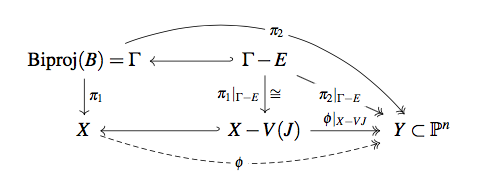
\includegraphics[scale=0.45]{graph.png}
\end{proof}
\end{frame}

% steps 2, 3
\begin{frame}
% \begin{proof}[Step 1 (cont)]
% 	\def\qedsymbol{}
% 	and we study the morphism $\pi_2$ instead of $\phi$.
% \end{proof}
\begin{proof}[Step 2]
	\def\qedsymbol{}
	Show that
	\[
		\ann_{\CC[\x]}((R/\I)_{\d,\bullet})=P
	\]
	and that
	\[
		\coker(N)\cong(R/\I)_{\d,\bullet}
	\]
	as graded modules over $\CC[\x]$.
\end{proof}
\begin{proof}[Step 3]
	\def\qedsymbol{}
	Construct an isomorphism between
	\[
		\Proj_{K(\CC[\x]/P)}(\CC[\x]-P)\inv(R/\I)
	\]
	and the scheme-theoretic inverse of the generic point $\gamma$ of the image $Y$
	\[
		\pi_2\inv(\gamma)=\Spec(\O_{\gamma,Y})\times_Y\Gamma(\phi)
	\]
\end{proof}
\end{frame}

% step 4 [finish]
\begin{frame}
\begin{proof}[Step 4]
	\def\qedsymbol{}
	Use the previous steps and a result from [Gelfand et al. [1994], A, Theorem 30],
	\[
		\ord_{Q(\mathbf x)}(\det(\mathcal{C}_\nbul))=\sum_i (-1)^i \mult_Q(H_i\mathcal{C}_\nbul)
	\]
	to get that
	\[
		\thediv(\det(\mathcal{C}_\nbul))=\length_{T_P}(B_{\d,\bullet})_P\cdot[Y]
	\]
	and finally, relate the latter length to the constant Hilbert polynomial of the preimage.
\end{proof}
\end{frame}



\section{The Algorithm}

\begin{frame}
\begin{lemma}
	Let $\{g_1,\ldots,g_k\}$ be a generating set for the Rees ideal $\I$ as an $\CC[\x]$-module,
	and let $({\mathbf a}_k,i_k)$ denote the bidegree of the $k$-th generator. Then the generators for
	$\I_{\d,\bullet}$ are given by
	\[
		\{s^\alpha g_k:{\mathbf a}_k+\alpha=\d:~\forall\alpha, k\}
	\]
\end{lemma}

\pause
\begin{algorithm}[non-Algorithm]
	\begin{itemize}
		\item compute a generating set for the Rees ideal $\I$
		\item use the above lemma to find the generators for $\I_{\d,\bullet}$
		\item construct $N$ out of the generators
		\item compute the minors
		\item compute the gcd
	\end{itemize}
\end{algorithm}
\end{frame}

% problems with examples 1 and 2
\begin{frame}
\begin{example}[Problem with bullet 1 in Example 2]
	\[
		\I=\Bigg\la
		\begin{cases}
		u {x}_{0}-s {x}_{1},
		(s v-101 u v) {x}_{2}+(-u t-u v){x}_{3},\\
		(t^{2}+t v) {x}_{1}-101 v^{2} {x}_{2}+(-t v-v^{2}) {x}_{3},\\
		(s t-101 ut) {x}_{1}-s v {x}_{3},v {x}_{0} {x}_{2}-101 v {x}_{1} {x}_{2}+(-t-v) {x}_{1}{x}_{3},\\
	  	t {x}_{0} {x}_{2}-101 t {x}_{1} {x}_{2}-101 v {x}_{2} {x}_{3}+(-t-v){x}_{3}^{2},\\
	  	s {x}_{0} {x}_{2}+(-202 s+10201 u) {x}_{1} {x}_{2}+(-s+101 u){x}_{1} {x}_{3}-s {x}_{3}^{2},\\
		t {x}_{0} {x}_{1}-101 t {x}_{1}^{2}-v {x}_{0}{x}_{3},\\P(x_0,x_1,x_2,x_3)
		\end{cases}\Bigg\ra
	\]
	In particular, $\I$ contains a lot of information not relavant to us.
	Worse than that, $P(\x)$ is always a generator of $\I$ in bidegree $(0,\deg(Y))$.
\end{example}
\begin{example}[Problem with bullet 3 in Example 1]
	In the case of $\d=2$, having a $6\times9$ one should {\bf not} compute all the minors,
	84 in this case, given that two random ones minors will often suffice.
\end{example}
\end{frame}

% algorithm - main
\begin{frame}
\begin{algorithm}[{\tt Main} - First Version]
\begin{algorithmic}
	\State{{\bf input:} none}
	\State{{\bf output:} the implicit equation $P$}
	\State{Set $r=\dim_\CC(S_\d)$}
	\State{Set $N'=r\times0$ matrix over $\CC[\x]$}
	\While{(Condition) is not satisfied for $N'$}
		\State{Given $N_1,\ldots,N_{i-1}$, use Algorithm {\tt LinearNi} to compute $N_i$}
		% \Comment{Call Recursion again}
		\State{Set $N'=N'~|~N_i$}
	\EndWhile
	\State{Report $P=\gcd(\minors(r, N'))$}
\end{algorithmic}
\end{algorithm}

\begin{itemize}
	\item[] (Condition) Given a matrix $N'$ and expected degree $k$, $N'$ is of full rank and there
	are nonzero minors of degree $\geq k$
\end{itemize}
\end{frame}

% algorithm - linear
\begin{frame}
\begin{algorithm}[{\tt LinearNi}]
\begin{algorithmic}
	\State{{\bf input:} a list of matrices of sygygy-generators $N_1,\ldots,N_{i-1}$}
	\State{{\bf output:} the syzygy-generators matrix $N_i$}
	\For{$0<j<i$}
	%	\State{Let $\mt{basis}(T)$ be the basis for $T_{i-j}$ as a row vector}
		\State{Set $N_{ji}=\mt{basis}(\CC[\x]_{i-j})\tensor N_{j}$}
		\State{Set $K_{ji}$ to be the linearization of $N_{ji}$}
	\EndFor
	\State{Set $K_i=\ker(\Phi^{(i)})$}
	\State{Let $K_i'$ be such that $\Span(K_i)=\Span(K_i')\oplus(\sum_j\Span(K_{ji}))$}
	\State{Let $N_i$ be such that $\mt{basis}(R_{\mathbf d,i})\cdot K_i'=\mt{basis}(S_{\mathbf d})\cdot N_i$}
	\State{Report $N_i$}
\end{algorithmic}
\end{algorithm}
\end{frame}

% degree 48 example
\begin{frame}
\begin{example}
	Let $X=(\PP^1)^3$ and let $\phi:X\To\PP^4$ be given by 5 general tri-cubics.
	Then $\phi$ is generically 1-1 and basepoint-free. Its image has degree $48=3!\cdot2^3$.
	This has far left the realm of Gr\"obner bases computations.
	
	\begin{itemize}
		\item do you really want the polynomial? --- dense on 270'725 monomials;
		\item
		at first one may hope that $\d=(1,1,1)$ is a good choice mimicing the results over $\PP^2$.
		Here $N$ will have $8$ rows and there will be no small-degree syzygies, so
		one can hope to get $N=N_6$ and $P(\x)=\det(N)$;
		\item there are no syzygies of degree $i$ over $S_\d$ for $i$ up to 10;
		\item any nonzero minor in the potential $N$ (whatever it is) will have degree at least 88;
		\item<2-> take another $\d$. for example, $\d=(2,2,1)$.
	\end{itemize}
\end{example}
\end{frame}

\begin{frame}
\begin{example}[cont]
	\begin{itemize}
		\item for $\d=(2,2,1)$ we have $r=18$ rows;
		\item it took 169 (0.03+1+19+147) seconds to find that $N_1=N_2=N_3=0$ and compute $N_4$;
		\item $N_4$ has $50$ columns, so a huge number of maximal minors;
		\item each nonzero minor of $N_4$ has degree $72>48$, so chances are that any two nonzero minors will do,
			as long as $N_4$ has any;
		\item it takes 3 second to check that $\rank N_4=18$;
		\item I grabbed two square submatrices $M_1$ and $M_2$ uniformly at random and checked if they are nonsingular
			by evaluating over a finite field. This took $0.2$ seconds; 
		\item at this point one has to make sure that $\det(M_1)$ and $\det(M_2)$ do not share common factor.
			this can be easily checked by hand -- see blackboard;
		\item it follows that $P(\x)=\gcd(\det(M_1),\det(M_2))$
	\end{itemize}
\end{example}
\end{frame}

\end{document}